\section{Measurement of external force at end effector} % \label{app:...}

As the Endowrist tool is highly nonlinear, measurement of how the end effector responds to external force should be made.

\subsection*{Purpose:}
To measure the relationship between the current and the force at the end-effector.

This test was made from engineering a simple setup where force could be measured. Therefore it should be noted that this test is not ideal as a load cell would have been preferable but it was not available. However it was possible to get a rough estimate of the relationship between current and force. 

The test setup can be seen on \figref{fig:Overview_force} 

\begin{figure}[H]
	\centering
	\begin{subfigure}{.45\textwidth}
		\centering
		\vspace{24pt}
		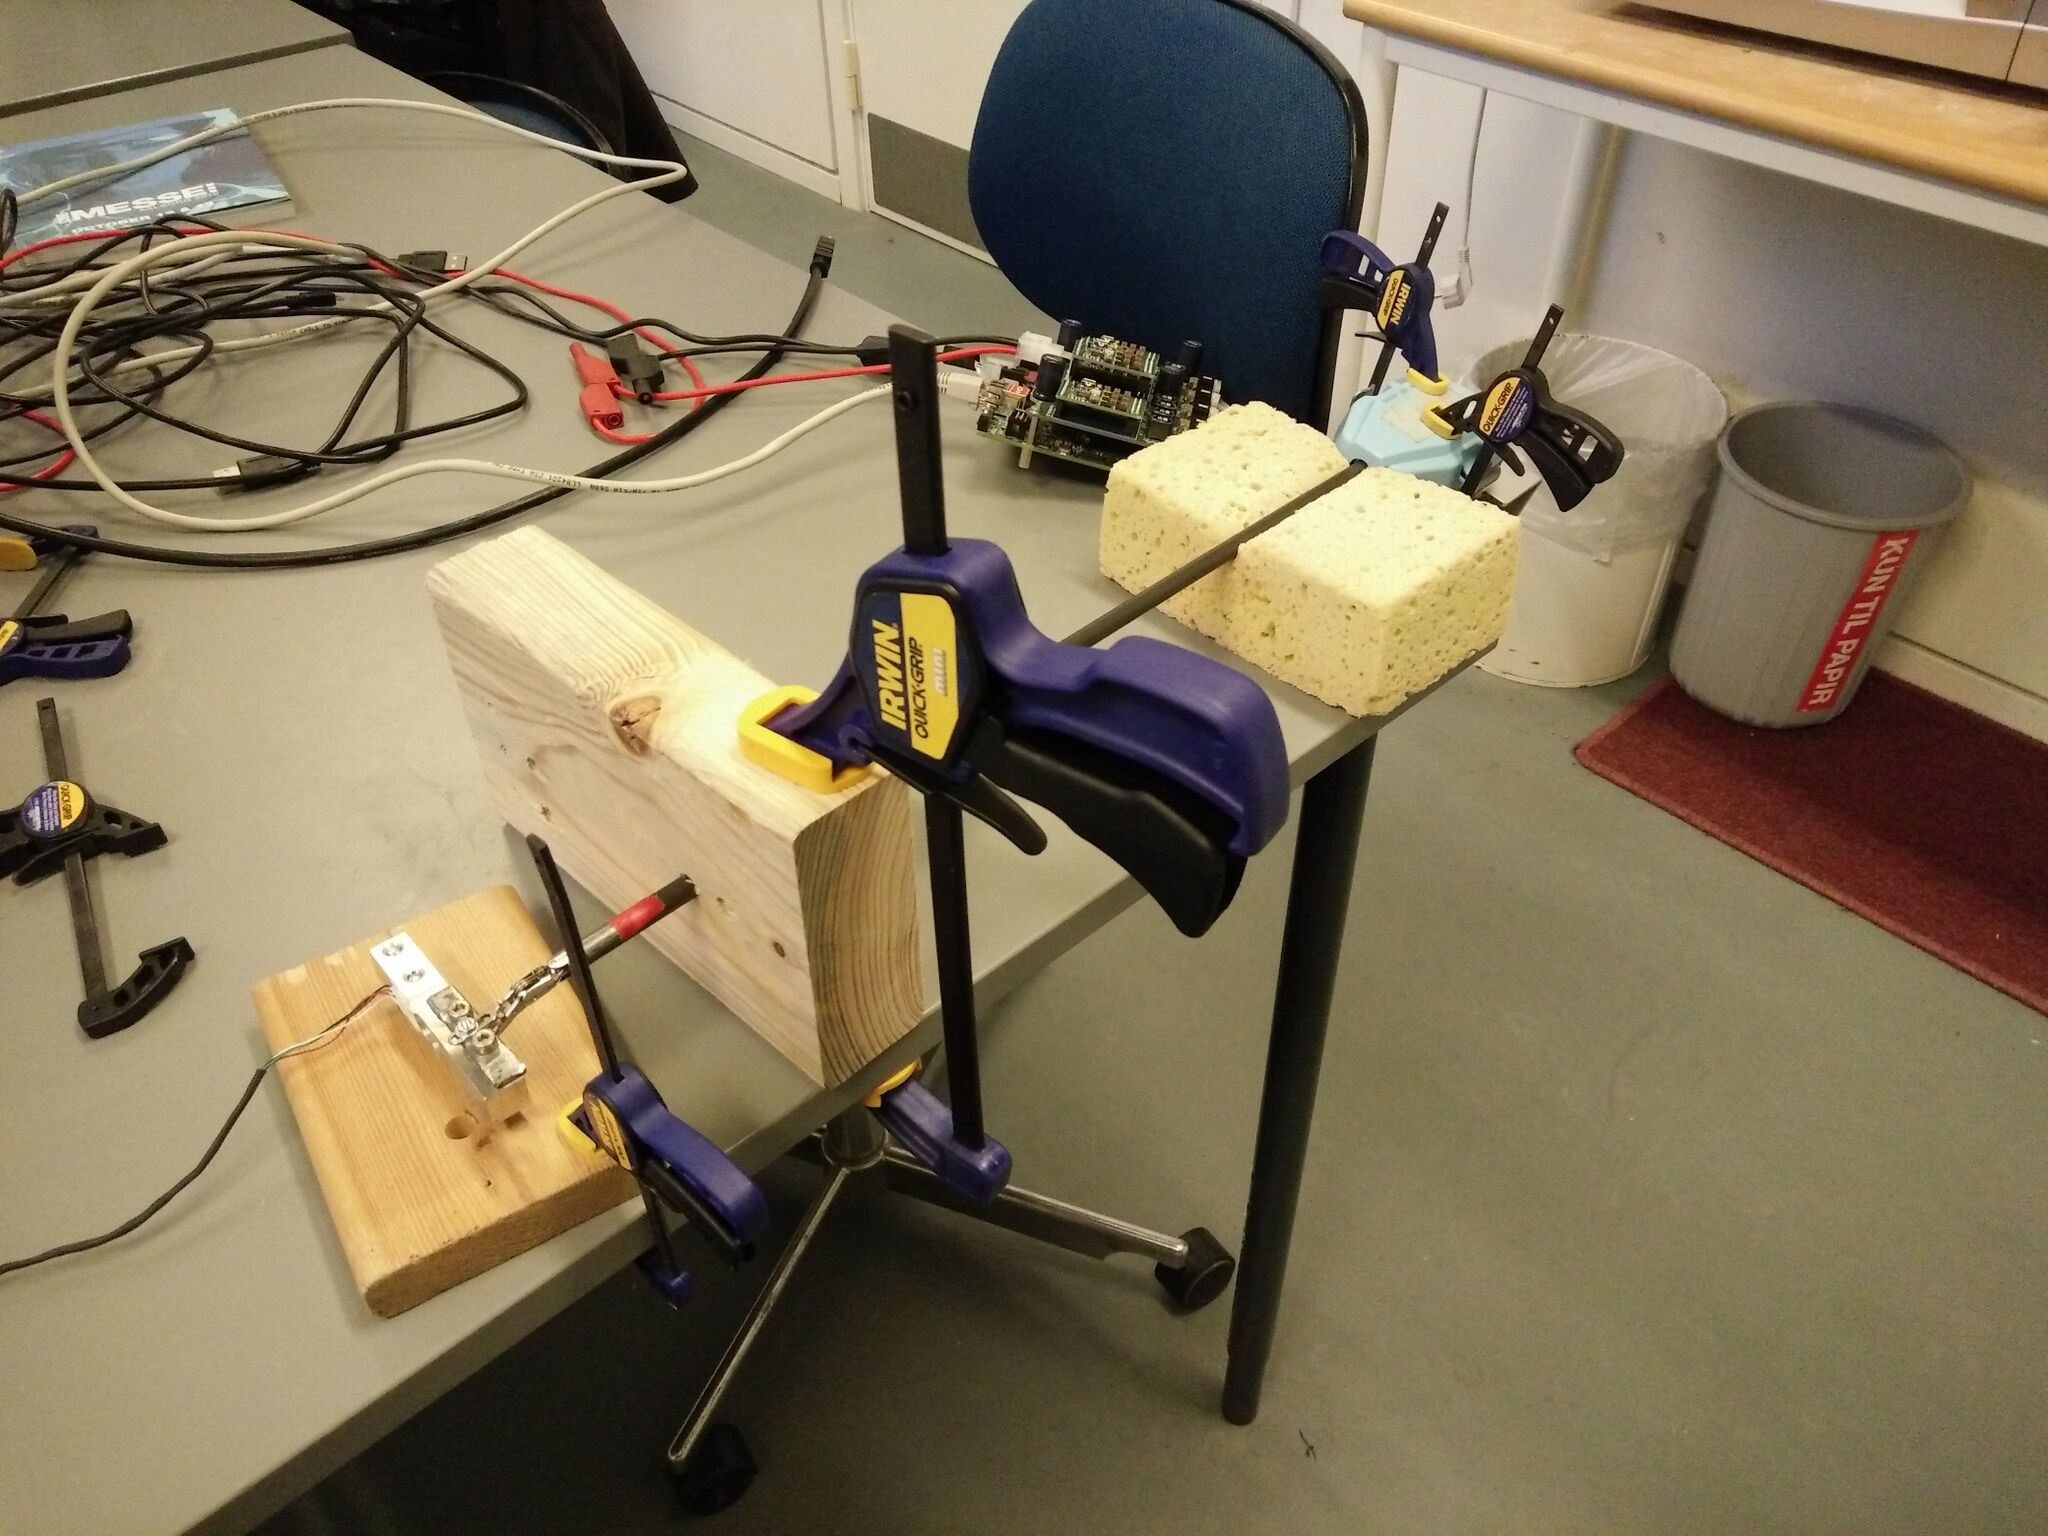
\includegraphics[width=\linewidth]{overall_force.jpg}
		\caption{The entire test setup. From the right, a scale for measuring the downwards force, a piece of wood for stiffening the Endowrist and keeping it it place and the Endowrist holder with motors.}
		\label{fig:entire_force_testsetup}
	\end{subfigure}
	\begin{subfigure}{.45\textwidth}
		\centering
		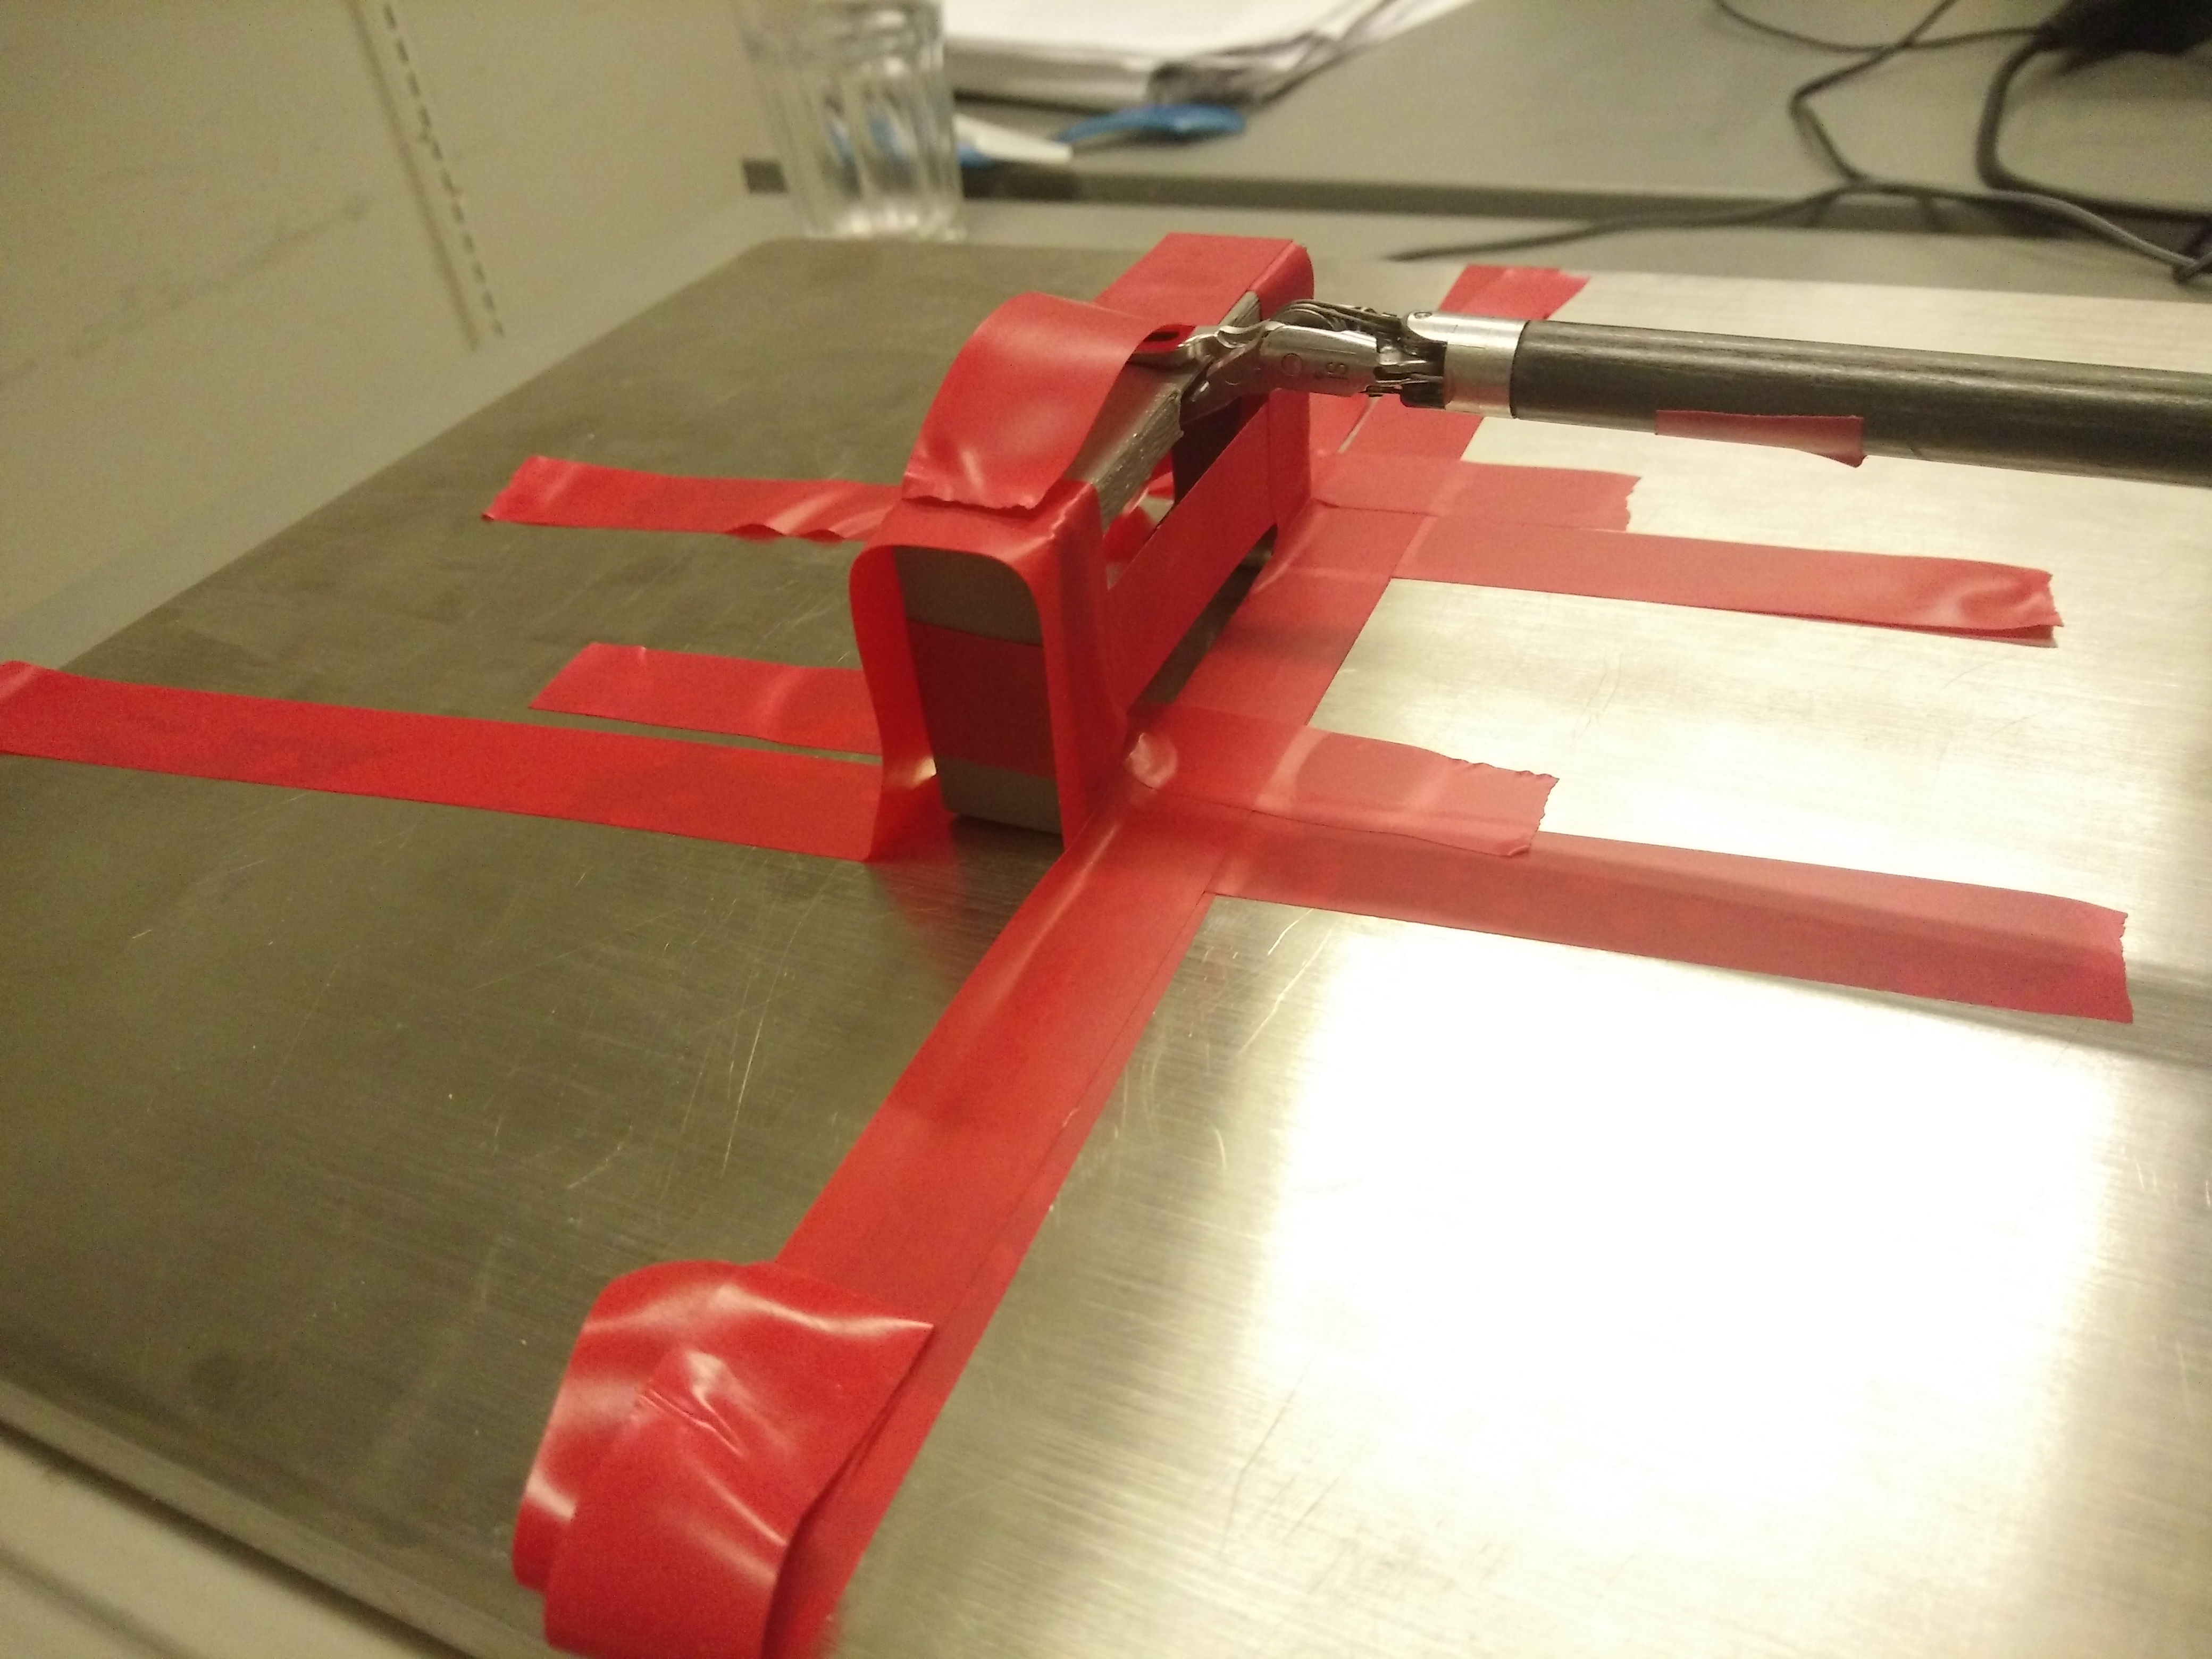
\includegraphics[width=\linewidth]{endeffector_force.jpg}
		\caption{A 3D printed case which made it possible to make an orthogonal force from the end-effector to the scale.}
		\label{fig:endeffector_force}
	\end{subfigure}
\caption{Test setup for the force estimation of the end-effector.}
\label{fig:Overview_force}
\end{figure}

\subsection*{Test equipment:}
\begin{itemize}
\item Endowrist model 420093 (AAU number: \#4).
\item Maxon 110160 motor with attached Maxon gearhead 110356 and Maxon encoder 201937.
\item Weight scale: Kern FCB 12K1 (AAU number: 86759).
\item Labview for measuring the current.
\item 3D printed case
\end{itemize}

\subsection*{Procedure:}
The following procedure was made for the force estimation:
\begin{enumerate}
\item The end-effector is set to an angle of $0^\circ$.
\item The end-effector was directly connected to the 3D printed case and taped to the scale.
\item The scale is reset to zero.
\item Current is increased to the motor which control the yaw of the end-effector, until first force measurement was available and noted.
\item Current is increased with approx. 50 - 100 mA and the force is noted in respect to the current until a current of 1 ampere is reached.
\end{enumerate}


\subsection*{Measuring data:}
The data from the measurements can be seen on \figref{endo_force_mes} A linear expression is made from the 340 mA sample and up and can be seen on \eqref{eq:linear_force_endo}.

\begin{equation}
\text{y} = 0.0028 \cdot \text{x} -0.8259 
\label{eq:linear_force_endo}
\end{equation} 



\subsection*{Results:}
It can be seen from the graph on \figref{endo_force_mes} that the force on the end-effector is highly nonlinear. The friction from the gearing and the Endowrist does that the force first begins to show around 200 mA due to the friction.


% This file was created by matlab2tikz.
%
%The latest updates can be retrieved from
%  http://www.mathworks.com/matlabcentral/fileexchange/22022-matlab2tikz-matlab2tikz
%where you can also make suggestions and rate matlab2tikz.
%
\definecolor{mycolor1}{rgb}{0.00000,0.44700,0.74100}%
\definecolor{mycolor2}{rgb}{0.85000,0.32500,0.09800}%
%
\begin{figure}[h]
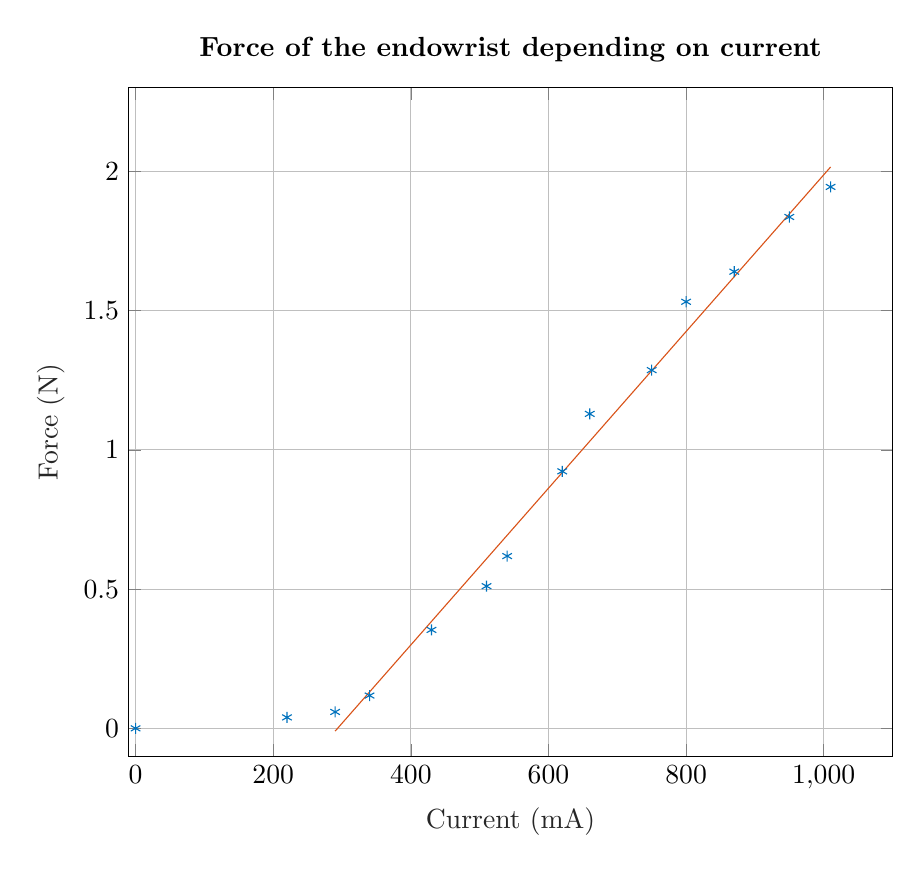
\begin{tikzpicture}

\begin{axis}[%
width=0.8\columnwidth,%7.484in,
height=0.7\columnwidth,%8.26in,
at={(0.758in,0.481in)},
scale only axis,
xmin=-10,
xmax=1100,
xlabel style={font=\color{white!15!black}},
xlabel={Current (mA)},
ymin=-0.1,
ymax=2.3,
ylabel style={font=\color{white!15!black}},
ylabel={Force (N)},
axis background/.style={fill=white},
title style={font=\bfseries},
title={Force of the endowrist depending on current},
xmajorgrids,
ymajorgrids
]
\addplot [color=mycolor1, draw=none, mark=asterisk, mark options={solid, mycolor1}, forget plot]
  table[row sep=crcr]{%
0	0\\
220	0.03928\\
290	0.05892\\
340	0.11784\\
430	0.35352\\
510	0.51064\\
540	0.61866\\
620	0.92308\\
660	1.1293\\
750	1.28642\\
800	1.53192\\
870	1.63994\\
950	1.83634\\
1010	1.94436\\
};
\addplot [color=mycolor2, forget plot]
  table[row sep=crcr]{%
290	-0.00996204344902341\\
340	0.130719594329395\\
430	0.383946542330548\\
510	0.609037162776017\\
540	0.693446145443068\\
620	0.918536765888537\\
660	1.03108207611127\\
750	1.28430902411242\\
800	1.42499066189084\\
870	1.62194495478063\\
950	1.8470355752261\\
1010	2.0158535405602\\
};
\end{axis}
\end{tikzpicture}%
\caption{The force measurements from the end-effector}
\label{endo_force_mes}
\end{figure}

\subsection*{Uncertainties of measurement:}
\begin{itemize}
\item Weight calibration.
\item Not 100 \% orthogonal force to the scale.
\item Elasticity of the 3D printed case, which made it possible for the end-effector to move a bit and get a slightly different angle than $0^\circ$. 
\item Movement of the entire setup when the elasticity of the 3D printed case reached a certain point.
\end{itemize}

\subsection*{Conclusion:}
It can be seen that the force on the end-effector has an exponential growth and is therefore not linear.
An estimation of a linear force increase is made from the 340 mA sample and up.\\
This test setup made it possible to make a rough estimate of the force at the end-effector. However this is not an ideal setup.

